\section{Architecture and data flow}
\label{sec:architecture}

Figure~\ref{fig:architecture} shows the system as the code builds it. It has three parts. The first
runs once and builds the index. The second runs for every question, in the web app or on the
command line. The third measures the second on a fixed question set. The source of the figure is
\code{docs/technical/architecture.dot}; \code{dot -Tpng -Gdpi=200} renders it to
\code{architecture_diagram.png}.

\begin{figure}[p]
  \centering
  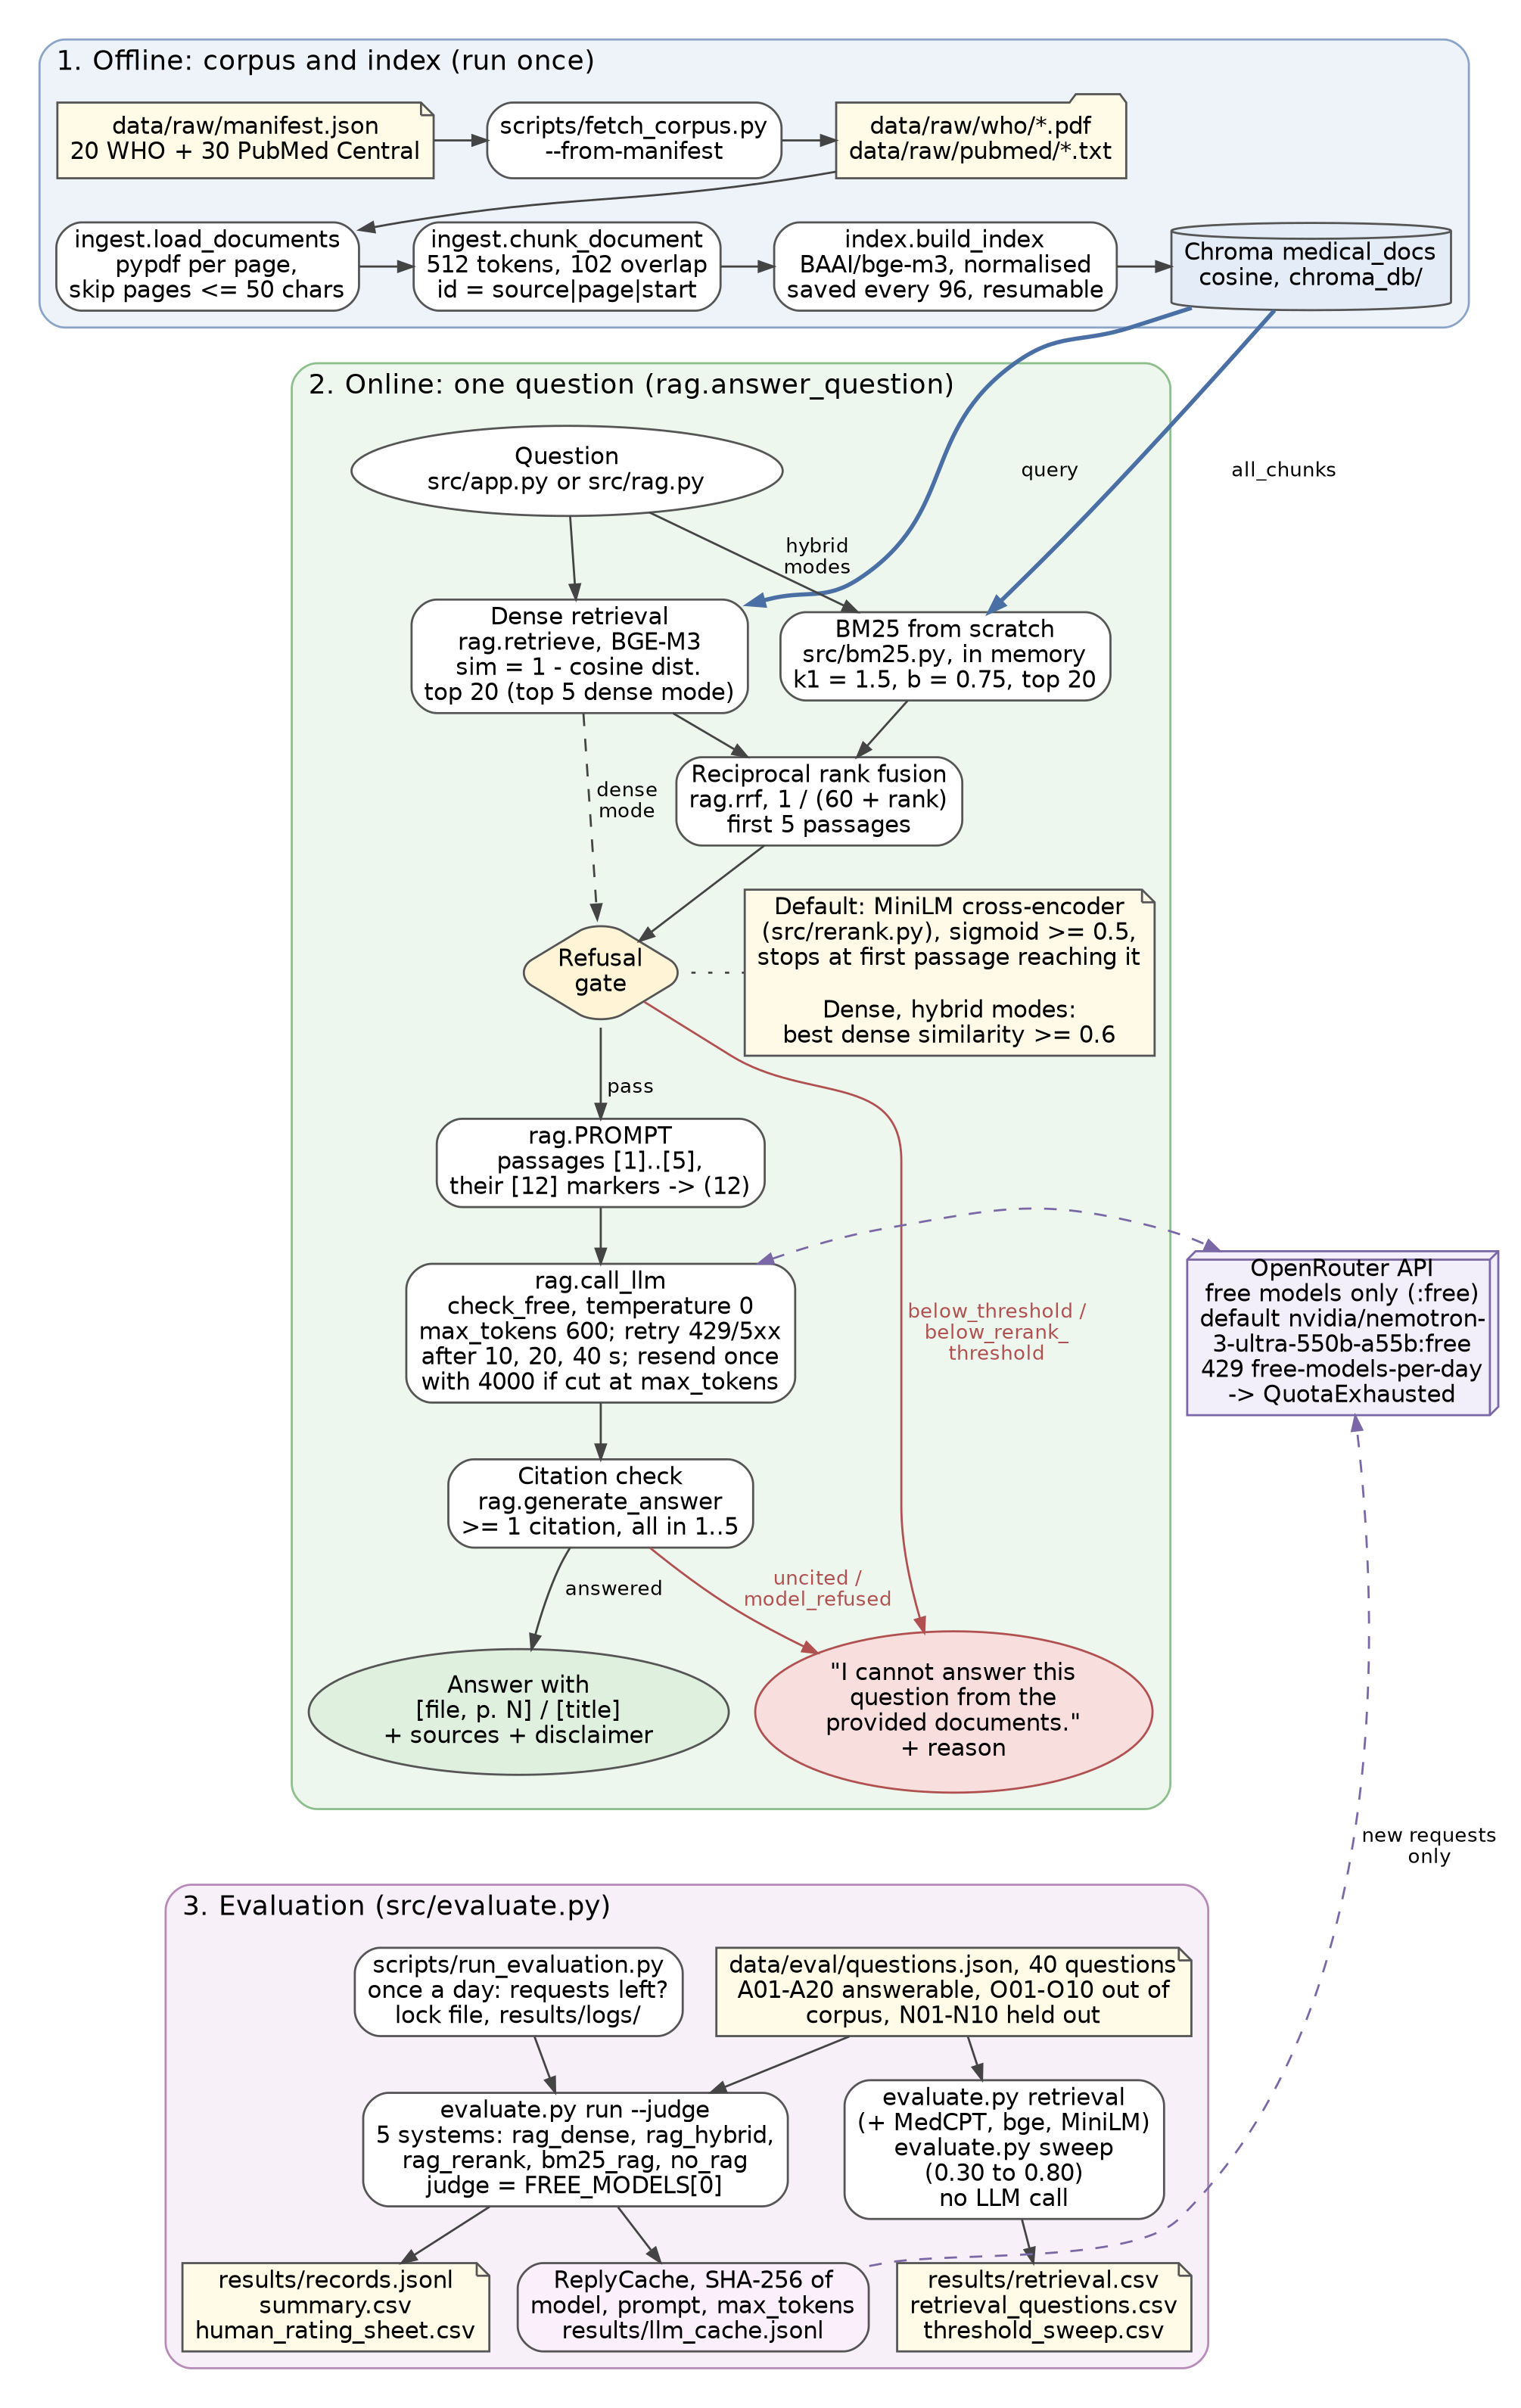
\includegraphics[height=0.9\textheight,width=\textwidth,keepaspectratio]{architecture_diagram.png}
  \caption{Architecture as built. Blue: offline indexing. Green: the path of one question, with
  its two refusal exits in red. Purple: the evaluation, which calls the same functions and sends
  every model request through a reply cache. Dashed purple arrows are network calls to OpenRouter.}
  \label{fig:architecture}
\end{figure}

\subsection{Offline: from documents to an index}

\begin{enumerate}[leftmargin=1.5em]
  \item The script \code{scripts/fetch_corpus.py}, run with \code{--from-manifest}, downloads the
        50 documents of the manifest (\nolinkurl{data/raw/manifest.json}): 20 WHO guidelines as PDF
        files from WHO IRIS, and 30 PubMed Central articles as plain text from the Europe PMC
        full-text API.
  \item \code{ingest.load_documents} reads each WHO PDF page by page with pypdf and skips pages of
        50 characters or fewer. Each PubMed article becomes one record with no page, cited by its
        title from the manifest.
  \item \code{ingest.chunk_document} cuts each record into windows of 512 tokens of the BGE-M3
        tokenizer, with 102 tokens of overlap, so a window moves by 410 tokens. A chunk keeps its
        source, page and kind. Its id is \code{source|page|start_token}.
  \item \code{index.build_index} embeds the chunks with \code{BAAI/bge-m3} (normalised vectors) and
        stores them in the persistent Chroma collection \code{medical_docs}, created with cosine
        distance. It saves every 96 chunks and, on a restart, only embeds the ids that are missing.
\end{enumerate}

\subsection{Online: one question}

\code{rag.answer_question} runs the whole path. The app offers three modes and the command line
has the same three (\code{--hybrid}, \code{--rerank}).

\begin{enumerate}[leftmargin=1.5em]
  \item \textbf{Retrieval.} The question is embedded with BGE-M3 and Chroma returns the nearest
        chunks; similarity is $1 - \text{cosine distance}$. In \emph{dense} mode the 5 nearest
        chunks are the passages. In the two hybrid modes, the 20 nearest chunks and the 20 best
        BM25 chunks are fused by reciprocal rank fusion and the first 5 are the passages. BM25 is
        built in memory at start-up from every chunk stored in Chroma, so both retrievers see the
        same chunks.
  \item \textbf{Refusal gate.} In \emph{dense} and \emph{hybrid} modes, the question is refused when
        the best dense similarity is below 0.6 (\code{SIM_THRESHOLD}). In the default mode,
        \emph{hybrid + cross-encoder gate}, the MiniLM cross-encoder scores the question with each
        passage, in retrieval order, and the question is refused when no passage reaches 0.5
        (\code{RERANK_THRESHOLD}) after a sigmoid. A refused question never reaches the model.
  \item \textbf{Generation.} The passages are numbered \code{[1]} to \code{[5]} under their source
        label, and the prompt asks a free model on OpenRouter to answer only from them, to cite a
        number after each claim, and to say the refusal sentence if the passages do not hold the
        answer. Reference markers inside the passages, such as \code{[12]}, are shown to the model
        as \code{(12)}.
  \item \textbf{Citation check.} The reply is kept only if it cites at least one passage and every
        cited number is between 1 and the number of passages. Each number is then replaced by a
        readable label, \code{[file, p. N]} for a WHO page or \code{[article title]} for a PubMed
        article. Otherwise, or if the model wrote the refusal sentence itself, the answer is the
        refusal sentence.
\end{enumerate}

Every result carries a reason, shown in the app under a refusal (Table~\ref{tab:reasons}).

\begin{table}[H]
  \centering\small
  \begin{tabularx}{\textwidth}{@{}l l X@{}}
    \toprule
    Reason & Set by & Meaning \\
    \midrule
    \code{answered} & \code{generate_answer} & Cited answer, every citation is a given passage. \\
    \code{below_threshold} & \code{answer_question} & Best dense similarity below the threshold; model not called. \\
    \code{below_rerank_threshold} & \code{answer_question} & No passage reaches the cross-encoder threshold; model not called. \\
    \code{uncited} & \code{generate_answer} & No citation, or a number outside 1..5. \\
    \code{model_refused} & \code{generate_answer} & The model wrote the refusal sentence. \\
    \code{no_context} & \code{generate_answer} & No passage was retrieved. \\
    \bottomrule
  \end{tabularx}
  \caption{The six reasons a result can carry.}
  \label{tab:reasons}
\end{table}

\subsection{Evaluation}

\code{src/evaluate.py} has three commands. \code{retrieval} and \code{sweep} make no model call:
they compare the retrievers and the gates on the question set and calibrate the similarity
threshold. \code{run} answers the question set with five systems (Section~\ref{sec:results}) and
writes one record per answer. It wraps \code{rag.call_llm} in a \code{ReplyCache}, so an identical
request (same model, prompt and token budget) is sent once and later reused.
\code{scripts/run_evaluation.py} runs one day's share of \code{run}, because the account allows 50
free-model requests a day.
